% chktex-file 10
\documentclass{article}
	\def\papertitle{Identifying regime transitions for water governance at a basin scale}
	\def\authors{Shuang Song, Shuai Wang*, Xutong Wu, Yongping Wei, Graeme S. Cumming, Yue Qin, Xilin Wu, Bojie Fu}
	\def\journal{Water Resources Research}
	\def\doi{\#2022WR033819}
% Define title defaults if not defined by user
\providecommand{\lettertitle}{Author Response to Reviews of}
\providecommand{\papertitle}{Title}
\providecommand{\authors}{Authors}
\providecommand{\journal}{Journal}
\providecommand{\doi}{--}

% For using tabularx
\usepackage{tabularx}
\usepackage{booktabs}
\usepackage[includeheadfoot,top=20mm, bottom=20mm, footskip=2.5cm]{geometry}

% Typography
\usepackage[T1]{fontenc}
\usepackage{times}
%\usepackage{mathptmx} % math also in times font
\usepackage{amssymb,amsmath}
\usepackage{microtype}
\usepackage[utf8]{inputenc}

% Misc
\usepackage{graphicx}
\usepackage[hidelinks]{hyperref} %textopdfstring from pandoc
\usepackage{soul} % Highlight using \hl{}

% Table

\usepackage{adjustbox} % center large tables across textwidth by surrounding tabular with \begin{adjustbox}{center}
\renewcommand{\arraystretch}{1.5} % enlarge spacing between rows
\usepackage{caption}
\captionsetup[table]{skip=10pt} % enlarge spacing between caption and table

% Section styles

\usepackage{titlesec}
\titleformat{\section}{\normalfont\large}{\makebox[0pt][r]{\bf \thesection.\hspace{4mm}}}{0em}{\bfseries}
\titleformat{\subsection}{\normalfont}{\makebox[0pt][r]{\bf \thesubsection.\hspace{4mm}}}{0em}{\bfseries}
\titlespacing{\subsection}{0em}{1em}{-0.3em} % left before after

% Paragraph styles

\setlength{\parskip}{0.6\baselineskip}%
\setlength{\parindent}{0pt}%

% Quotation styles


% Quotation styles
\usepackage{framed}
\usepackage{xkeyval} % To define custom key-value pairs

\makeatletter
% Define the keys
\define@key{myquote}{page}{\def\mypage{#1}}
\define@key{myquote}{sline}{\def\mysline{#1}}
\define@key{myquote}{eline}{\def\myeline{#1}}
\presetkeys{myquote}{page=Unknown, sline=Unknown, eline=}{}

\let\oldquote=\quote
\let\endoldquote=\endquote
\renewenvironment{quote}[1][]{%
    \setkeys{myquote}{#1}% Process the keys
    \begin{fquote}
    \ifx\myeline\empty
        \noindent\textbf{Page: \mypage, Line: \mysline} \\
    \else
        \noindent\textbf{Page: \mypage, Line: \mysline\textasciitilde\myeline} \\
    \fi
    \advance\leftmargini -2.4em
    \begin{oldquote}
}{
    \end{oldquote}
    \end{fquote}
}
\makeatother


\usepackage{xcolor}
\newenvironment{fquote}
  {\def\FrameCommand{
	\fboxsep=0.6em % box to text padding
	\fcolorbox{black}{white}}%
	% the "2" can be changed to make the box smaller
    \MakeFramed {\advance\hsize-2\width \FrameRestore}
    \begin{minipage}{\linewidth}
  }
  {\end{minipage}\endMakeFramed}

% Table styles

\let\oldtabular=\tabular
\let\endoldtabular=\endtabular
\renewenvironment{tabular}[1]{\begin{adjustbox}{center}\begin{oldtabular}{#1}}{\end{oldtabular}\end{adjustbox}}


% Shortcuts

%% Let textbf be both, bold and italic
%\DeclareTextFontCommand{\textbf}{\bfseries\em}

%% Add RC and AR to the left of a paragraph
%\def\RC{\makebox[0pt][r]{\bf RC:\hspace{4mm}}}
%\def\AR{\makebox[0pt][r]{AR:\hspace{4mm}}}

%% Define that \RC and \AR should start and format the whole paragraph
\usepackage{suffix}
\long\def\RC#1\par{\makebox[0pt][r]{\bf RC:\hspace{4mm}}\textbf{\textit{#1}}\par} %\RC
\WithSuffix\long\def\RC*#1\par{\textbf{\textit{#1}}\par} %\RC*
\long\def\AR#1\par{\makebox[0pt][r]{AR:\hspace{10pt}}#1\par} %\AR
\WithSuffix\long\def\AR*#1\par{#1\par} %\AR*


%%%
%DIF PREAMBLE EXTENSION ADDED BY LATEXDIFF
%DIF UNDERLINE PREAMBLE %DIF PREAMBLE
\RequirePackage[normalem]{ulem} %DIF PREAMBLE
\RequirePackage{color}\definecolor{RED}{rgb}{1,0,0}\definecolor{BLUE}{rgb}{0,0,1} %DIF PREAMBLE
\providecommand{\DIFadd}[1]{{\protect\color{blue}\uwave{#1}}} %DIF PREAMBLE
\providecommand{\DIFdel}[1]{{\protect\color{red}\sout{#1}}}                      %DIF PREAMBLE
%DIF SAFE PREAMBLE %DIF PREAMBLE
\providecommand{\DIFaddbegin}{} %DIF PREAMBLE
\providecommand{\DIFaddend}{} %DIF PREAMBLE
\providecommand{\DIFdelbegin}{} %DIF PREAMBLE
\providecommand{\DIFdelend}{} %DIF PREAMBLE
%DIF FLOATSAFE PREAMBLE %DIF PREAMBLE
\providecommand{\DIFaddFL}[1]{\DIFadd{#1}} %DIF PREAMBLE
\providecommand{\DIFdelFL}[1]{\DIFdel{#1}} %DIF PREAMBLE
\providecommand{\DIFaddbeginFL}{} %DIF PREAMBLE
\providecommand{\DIFaddendFL}{} %DIF PREAMBLE
\providecommand{\DIFdelbeginFL}{} %DIF PREAMBLE
\providecommand{\DIFdelendFL}{} %DIF PREAMBLE
%DIF END PREAMBLE EXTENSION ADDED BY LATEXDIFF

\usepackage{xr-hyper}
% 参考其它文件的标签 https://texfaq.org/FAQ-extref
\usepackage{xr}
\externaldocument[SI]{../sup/supplementary_information}
\externaldocument[MS]{../main/manuscript}

\begin{document}

% Make title
{\Large\bf \lettertitle}\\[1em]
{\huge \papertitle}\\[1em]
{\authors}\\
{\it \journal, }\texttt{\doi}\\
\hrule

% Legend
\hfill {\bfseries RC:} \textbf{\textit{Reviewer Comment}},\(\quad\) AR\: Author Response, \(\quad\square\) Manuscript text


\graphicspath{{/Users/songshgeo/Documents/VSCode/WGRegimes_YRB_2020/figures/}}

\section{Associate Editor}

\subsection{General comments}
\RC{} Dear Authors, thanks for the submission of the manuscript. We have asked two experts in the relevant fields to review the manuscript. Both reviewers overall find the merit in the manuscript however they also noted several major issues in the current manuscript. With my own reading, I fully agree with the reviewers and would like to highlight a few major issues:

\AR{} Thank you for your constructive comments and for providing us with the opportunity to address the concerns raised by both reviewers. We appreciate the valuable feedback, which has helped us identify areas for improvement in our manuscript. We have carefully considered each point and have made substantial revisions to address these issues. Please find our detailed responses to the highlighted concerns below.

\subsection{Issue \#1}
\RC{} overall the results and discussion are relatively shallow and I would encourage the authors to do deep dive into the results, e.g.\ change points, as also pointed out by both reviewers,

\AR{} We acknowledge the need for a more in-depth analysis of our results. We have re-evaluated our data and expanded the results and discussion sections to include a deeper dive into the findings, specifically regarding the change points mentioned by both reviewers. We have also provided more context and explanation for these changes in the manuscript, which can be found on pages 14\-16 and 18\-21.

\subsection{Issue \#2}
\RC{} I fully agree with Reviewer \#2 that more thorough review of existing and relevant indicators with IWGI,

\AR{} We agree with Reviewer \#2's suggestion to include a more thorough review of existing and relevant indicators with IWGI. We have added a new section in the manuscript discussing these indicators, comparing and contrasting their strengths and weaknesses, and explaining how our approach fills the gaps in the current literature. This new section can be found on pages 5\-7.

\subsection{Issue \#3}
\RC{} I would encourage the authors to look into more recent data (beyond 2013) as pointed out by Reviewer 1. In addition, I find the data in supplementary materials is not accessible, which should be amended. The data access and reproduction of the methodology/results are very important for WRR and our scientific community, so we take the issue related with data accessibility very seriously.

\RC*{} Overall, based on the reviewers' recommendations, I would like to ask the authors to submit a suitably revised manuscript in due course.

\AR{} We appreciate the importance of using up-to-date data in our research. We have now included more recent data in our analysis, extending our dataset up to 2021. The updated data, along with the revised results and discussion, can be found on pages 11-13 and 18-21.

\AR*{} We apologize for the inconvenience caused by the inaccessibility of the supplementary materials. We have rectified this issue by ensuring that all supplementary data and files are now accessible and properly linked within the manuscript. We have also provided a clear description of the data and methodology in the supplementary materials to facilitate reproducibility of our results.

\AR*{} We hope that these revisions address the concerns raised by both reviewers and the associate editor. We are confident that these changes have significantly improved the quality of our manuscript and made it more relevant and valuable to the scientific community. We look forward to your further feedback and the possibility of our manuscript being accepted for publication.

\newpage
\section{Reviewer \#1}

\subsection*{Overall comments} % todo

\RC{} This study proposed an integrated index that incorporates water resources, water use, and water allocation to represent the water governance regime in the Yellow River basin. The authors showed an in-depth understanding of the water governance in this basin and made a great effort to represent the status of water governance straightforwardly with the integrated index. The figures were generally well-designed and presented clearly. But I feel the paper lacks details of the results which makes it difficult to understand the paper. Specific comments are listed below.

% 感谢您认可。
% 很抱歉缺少细节,可能会使您难以完全理解我们的研究。
% 为了回应您的担忧,我们已经修改了我们的稿件,并提供了更详细的结果解释。请在下面找到我们对您的具体评论的逐条回复。
\AR{} Thank you for your valuable feedback and for acknowledging our efforts in understanding the water governance in the Yellow River basin. We appreciate your comments regarding the clarity of the figures and our integrated index. Sorry about the lack of details in the results section may have made it difficult to fully comprehend our study. In response to your concerns, we have revised our manuscript and provided a more detailed explanation of the results. Please find our point-by-point response to your specific comments below.

\subsection{Major concern \#1}

% 气候变化在指数中没有明确的体现,这可能是本世纪黄河流量恢复的关键因素。气候变化将是未来该流域面临的巨大挑战。重大的气候变化可能影响流域的适应能力,因此需要不同的治理策略。
\RC{} Climate change is not explicitly represented in the index, which might play a key role in the streamflow recovery in the Yellow River in this century. Climate change would be a great challenge in the basin in the future. Significant climate change may affect the adaptive capacity of a basin and thus require different governance strategies.

% 气候变化的确会产生很多影响,例如改变降水量和蒸发量。但这些影响都会以影响可用水量的形式体现在IWGI之中。
% 在新增加的图表中,我增加了天然水量的图表展示这种变化
% 例如气候变化让可用水量发生改变(scarcity),极端气候让我们难以有效的分配水资源(allocation),对气候变化的适应可能导致社会变革,让人们对愈发侧重于工业和经济发展的治理策略进行反思(priority)。
% 我们现在在讨论中涉及了这些话题。
\AR{} Climate change indeed has a multitude of impacts, such as altering precipitation and evaporation rates.
However, these effects are inherently captured within the Integrated Water Governance Index (IWGI) as they influence the available water resources.
In the revised version of our paper, we have added new graphs to demonstrate the changes in natural water availability caused by climate change.
For example, climate change may alter water scarcity levels and make it more difficult to effectively allocate water resources due to extreme climate events.
Additionally, adapting to climate change could lead to societal transformations, prompting a reevaluation of governance strategies that increasingly focus on industrial and economic development (priority).
We have now addressed these topics in our discussion, illustrating the various ways in which climate change influences the adaptive capacity of a basin and its subsequent governance requirements.

\begin{quote}
	Climate change may alter water scarcity levels and make it more difficult to effectively allocate water resources due to extreme climate events.
\end{quote}

\begin{figure}[!htb]
	\centering
	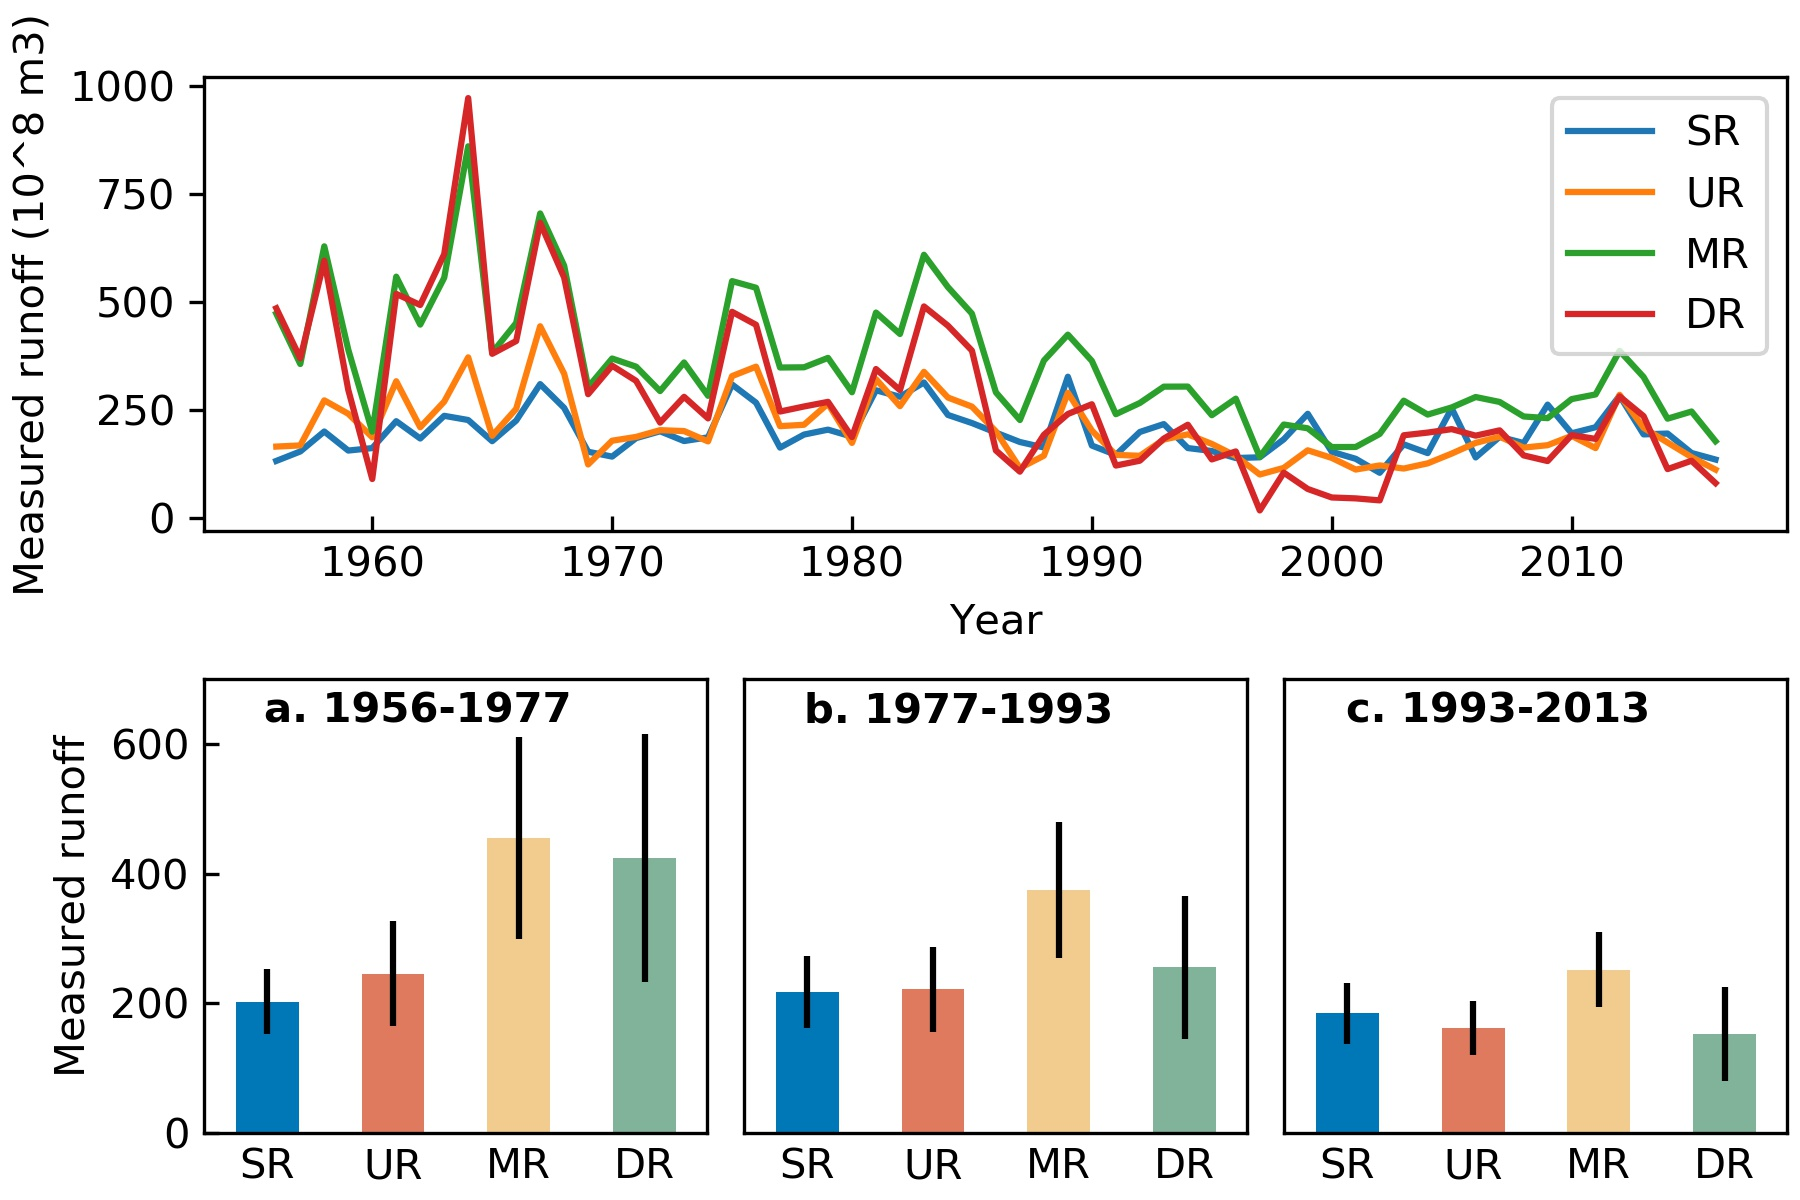
\includegraphics[width=\textwidth]{sup/sf_measured_runoff.jpg}
	\caption{绘图测试}\label{fig:xfig0}
\end{figure}

% 我们强调流域治理需要考虑这些因素,但我们可能很难穷尽优秀的流域治理策略需要考虑哪些因素。因此,IWGI至少让我们可以知道在诸多治理因素的共同影响下,流域的未来正在走向何方。
\AR*{}

\subsection{Major concern \#2}
% 结果是总结性的。我建议提供更多关于三个指数和IWGI结果的信息。例如,三个指标的结果,以及分区域的结果。请解释IS、IP、IA和IWGI这三个指标的范围,以及不同数值的含义。这些细节可以帮助读者理解结果的合理性。
\RC{} The results are summative. I would suggest providing more information on the results of the three indices and the IWGI.\ For example, the results of the three indices, and the results for the sub-regions. And please explain the range of the three indicators, IS, IP, IA, and the IWGI, and the meanings of different values. These details could help readers understand the reasonability of the results.

\subsection{Major concern \#3}
% 本研究中使用的数据似乎有不同的时间段,大多数数据来自2013年之前。近十年来,黄河的水文状况和水治理应该发生了重大变化。因此,结合近十年的结果将使这项研究更加可靠。
\RC{} The data used in this study seem to have different time periods, and most data are from before 2013. The hydrological regime and water governance in the Yellow River should have changed significantly in the recent decade. Therefore, incorporating the result from the recent decade would make this study more solid.

\subsection{Major concern \#4}
% 这三个指标之间可能存在相互作用/相互联系。作者是否检查了指标之间的关系?
\RC{} There might be interactions/interconnections among the three indicators. Did the authors examine the relations between the indicators?

\subsection{Major concern \#5}
% IWGI在“应力”方面包含储层存储信息。输水能力是衡量水治理/水社会复原力的重要指标。
\RC{} The IWGI includes reservoir storage information in the "stress" aspect. However, the water conveyance ability is not represented, which is also an important indicator of water governance/hydrosocial resilience.

\subsection{Major concern \#6}
% 我建议在标题中加上“黄河流域”。因为没有对IWGI的适用性和有效性进行测试或讨论。它能在其他盆地使用吗?使用索引的先决条件是什么?
\RC{} I would suggest adding "Yellow River basin" in the title. Because the applicability and validity of the IWGI were not tested or discussed. Can it be used in other basins? What is the prerequisite for using the index?

\subsection{Major concern \#7}
% 最好在引言部分解释“水治理机制”的概念,然后解释使用综合指数IWGI代表水治理机制的必要性。
\RC{} It would be better to explain the concept "water governance regime" in Introduction and then explain the necessity of using the integrated index IWGI for representing the water governance regime.
\subsection{Detailed issues}

% 我没有在引用的文献中找到“用水的三个核心方面”。这三个方面是作者提出的吗?
\RC{} Line 57-62: I did not find the "three core aspects of water use" in the cited reference. Were the three aspects put forward by the authors?

\RC{} Line 92: missing information for the citation?

\RC{} Line 94-95: the sentence is unclear.

\RC{} Line 121: Repeated citation Qin et al. 2019.

\RC{} Line 122: It would be better to introduce the calculation of SFV in the main text.

\RC{} Equation (6): Why is the numerator WUpro not WUnon-pro? Please check the equation.

\RC{} Equation (7): CEM => AEM?

\RC{} Line 154: Please explain the source of irrigated area data.

\RC{} Fig.2A, p<0.01 or p<0.001? (line 147 says that α=0.001 was used for the change-point detection).

\RC{} Fig.2C: How were the directions determined?

\RC{} Fig.3C: What do the dashed lines denote?

\RC{} Line 187: what is "social transformation"?

\RC{} Line 208: the IWGI was proposed in this study, here the citations of Loch's and Turton's studies are not appropriate.

\RC{} Line 273: adapted => adopted?

\RC{} Line 275: biophysical? Please check the sentence.

\newpage
\section{Reviewer \#2}

\subsection*{Overall comments}
% 作者提出了IWGI,并将其应用于黄河流域的水治理历史,分析了流域的制度变迁。该方法具有很强的合理性和适应性,案例分析的结果为理解中国的水治理提供了有益的见解。然而,讨论并没有充分利用案例研究分析的结果。讨论结果的内容应该更具有支持性和可靠性。此外,讨论的叙事分析非常有趣,但如果这项研究的原创性之一是识别变化点,那么就需要更多地讨论导致这些变化点的触发因素。请参考我下面的审稿意见并进行修改,以提高本文的价值。
\RC{} The authors proposed the IWGI, applied the index to the history of water governance in the Yellow River basin, and analyzed the regime change in the basin. The methodology is very reasonable and adaptable, and the results of the case analysis provide useful insights for understanding water governance in China. However, the discussion does not fully exploit the results of the case study analysis. The discussion should be more supportive and solid in its content of the results. Also, the narrative analysis of the discussion is very interesting, but if one of the originalities of this study is the identification of change points, more discussion of the triggers that caused these change points is needed. Please refer to my review comments below and revise them to enhance the value of this paper.

\AR{} Thanks!

\subsection{Comment \#1}
% 图1:很难理解B中每个数字的含义。也许是这个数字的大小有问题。
\RC{} Figure 1: It is difficult to understand what each number in B means. Perhaps it may be a problem with the size of the figure.

\subsection{Comment \#2}
% 导言:与流域和水资源相关的指标有很多,其中一些指标具有与治理和政策相关的参数。为了突出你所制定的IWGI的新颖性,也许你可以加上对其他相关指标的审查。
\RC{} Introduction: There are many indicators related to watersheds and water resources, some of which have parameters related to governance and policy. To highlight the novelty of the IWGI that you have developed, perhaps you could add a review of other relevant indicators.

\subsection{Comment \#3}
% 方程:方程(7)中的CEM是什么?还有,水的比例指的是什么?支持信息中公式(2)中的一些术语没有解释。例如:R或WU。
\RC{} Equations: what is the CEM in equation (7)? Also, what does the water proportion refer to? Some of the terms in equation (2) in Supporting Information are not explained. e.g. R or WU. 

\subsection{Comment \#4}
% 第2.2节:您提到您将Pettitt(1979)方法应用于“水文时间序列”,但结果似乎适用于IWGI时间序列数据。请说明您将该方法应用于哪些数据。
\RC{} Section 2.2: You mention that you apply the Pettitt (1979) approach to "hydrological time series", but the results appear to be for IWGI time series data. Please clarify to which data you applied the approach.

\subsection{Comment \#5}
% 图3:D中哪些类型的官方文件被统计以及如何统计?
\RC{} Figure 3: What types of official documents in D are counted and how?

\subsection{Comment \#6}
% 讨论:每个政权的故事都令人印象深刻。然而,结果与图3的关系并不清楚。请通过更直接地引用结果和图3来加强你的论点。
\RC{} Discussion: The stories of each regime are very impressive. However, the relation to the results and Figure 3 is not clear. Please strengthen your argument by citing the results and Figure 3 more directly.

\subsection{Comment \#7}
% 讨论:从您对变更点的分析中可以明显看出,每个制度中都存在变更点。但为什么会出现这些变化“点”呢?是什么导致或触发了它们?这是管理机构的变化还是象征性的政策变化?该制度期间的特征已被很好地描述,但请更多地考虑为什么变化点发生在特定的年份/时期。
\RC{} Discussion: The existence of change points in each of the regimes is evident from your analysis of the change points. But why did these change "points" occur? What caused or triggered them? Was it a change in governing institutions or a symbolic policy change? The characteristics during that regime period are well described, but please give more thought to why the change points occurred in that particular year/period.

\subsection{Comment \#8}
% 图4:A中的蓝色圆形箭头和B中的红色圆形箭头是什么意思?它们似乎包含了您非常重要的言论,但它们并不清楚。此外,您需要更多地解释A和B中的每个箭头。
\RC{} Figure 4: What do the blue circular arrows in A and the red circular arrows in B mean? They seem to contain your very important remarks, but they are unclear. Also, you need to explain more about each of the arrows in A and B.

\subsection{Comment \#9}
% 结论:对定量分析的结果进行了描述,但是Discussion中的叙事分析似乎没有得到充分的体现。建议对此添加几行。
\RC{} Conclusion: The results of the quantitative analysis are described, but the narrative analysis in the Discussion does not seem to be fully reflected. It is recommended to add a few lines about it.

\end{document}
